\section{Experiments}
\label{sec:experiments}
This section is on data analysis by detailing the three main steps described in section \ref{sec:introduction}. The main goal is to find the differences of CST in a healthy brain and a ALS (Amyotrophic Lateral Sclerosis) diseased brain based on quantification some metric values. 

%definition of ALS
%copy and paste from ~\cite{horsfield2002applications}
ALS, also known as motor
neurone disease and Lou Gehrig’s disease, is a fatal,
progressive neuromuscular disease that attacks the motor
neurons controlling voluntary movement. The result is
wasting and atrophy of muscles, leading to difficulties in
speaking or swallowing, stumbling, permanent fatigue
and cramping, amongst other symptoms. The frequency
is about 6 per 100 000. ALS can be broadly classified into
two groups—bulbar onset and limb onset—depending on
how symptoms first manifest themselves. The first
symptoms of bulbar onset ALS include speaking and
swallowing difficulties, resulting from degeneration of
motor neurons concentrated in the brain stem (cortico-
bulbar region). Limb onset patients experience first
symptoms of ALS as muscle weakness in either the arms
or legs. Limb onset patients eventually experience bulbar
symptoms as the disease progresses.
The first study of ALS using diffusion-weighted
imaging was by Segawa et al.26 who, although observing
differences in T2—weighted images in ALS patients (i.e.
hyperintense lesions), did not find any significant
diffusion changes in the posterior limb of the internal
capsule of ALS patients. Wu et al.27 demonstrated
hyperintensity in diffusion-weighted images (signifying
reduced diffusivity) in the cortico-spinal tracts in 11 of 12
ALS patients and five of 12 controls. However, since
diffusion-weighting was only applied in one direction
(left–right) it is likely that this study was confounded by
the effects of diffusion anisotropy.~\cite{horsfield2002applications}


\subsection{Tractography Reconstruction}
\label{subsec:experiments_reconstruction}
This first part will describes how to create the tractography from the raw data in DICOM format. After that, the validation of the tractography is also presented.
\subsubsection{Preprocessing}
The content of this part is from the technical report \cite{bao2012dmri}. In general, in order to perform tractography from discrete measured diffusion tensor MRI data, there are some steps as follow:

\begin{enumerate}
\item From raw data to Nifti format.
\item Reconstruction.
\item Tracking.
\item Coregistration.
\end{enumerate}

The first step is to convert from DICOM to Nifti format. End of this step, all the necessary information for tracking have been extracted from the DICOM raw data including: actual dMRI data (4D array, $(I,J,K,W)$), affine transformation, gradient vector ($‘.bvec’$) and b-value ($‘.bval’$).
From these information,we can create the \emph{tractrography}, the \emph{fractional anisotropy} (FA) volume and the \emph{mean diffusivity} (MD) volume.
A tractography is created in two steps: reconstruction and tracking. Reconstruction is about computing the information about the spatial distribution of the diffusion signal within each voxel. While tracking tries to connect many signals to form a tractography based on orientation signal of each voxel. In this paragraph, the main focus is on how to reconstruction of dMRI data.   

However, before doing reconstruction, the actual dMRI data in NIfTI image needs to extract brain image only. Because the result of scanner usually contains not only brain but also other things close to brain which can distract the processing of tracking. Brain extraction is the process of removing the skull and the rest of the head from the brain, therefore is necessary to be done before further analysis. The resulting file only contains a representation of the brain's anatomy. Brain extraction can be done with the FSL program BET (Brain Extraction Tool)~\cite{smith2002automated}. FSL\footnote{\url{http://www.fmrib.ox.ac.uk/fsl/index.html}} is a comprehensive library of analysis tools for FMRI, MRI and DTI brain imaging data.

After creating tractographies from the raw data in dicom format, the next step is coregistration. Becasue all these tractographies were initially in native space or space of scanner and every measurement has it own coordinator, it is very difficult for doctor or neuroscientist can compare, integrate or further studying them. They are needed to be warped into the common space. The goal is to warp the tractography from native space into MNI space (Montreal Neurological Institute)~\footnote{\url{http://www.mni.mcgill.ca/}}, a standard brain based on the averaging of 58 peoples. In contrast to the all the method mentioned before, in this implement we use FA registration mappings or affine transformation applied on tractography which is also most commonly used in the literature along with other tensor based methods~\cite{goh2006algebraic}. More detail can be found in \cite{bao2012dmri}

At the end of this procedure, we get the whole tractography in the common MNI cordinator. The next step is to validate the result to check the accuracy of the tractography.

\subsubsection{Validation}
This step is aimed at validation the result tractography of the previous step. We investigate on two ways. First, we try to statistic analyse the tractography of all subjects and controls to see whether there is any unusual case or not. Some features can be used such as

\begin{enumerate}
	\item Number of tracts for every subject and control
	\item Length: min, max and average
	\item Align on spagetti
\end{enumerate}

%
\includepdf[pages={1-3},picturecommand={Statistical features of the tractography}]{validation_120531_dti_10k.pdf}
\label{table:validation}

%\begin{figure}  
%  \centering
%  \includegraphics[width=15cm]{validation_120531_dti_10k.pdf}
%  %[bb 0 0 400 400]
%  \caption{The statistical features of tractography.}
%  \label{fig:validation}
%\end{figure}
%
The table in the \ref{table:validation} shows the statistic of some basic features of tractography. Note that, here we use $10K$, $1M$ and $3M$ seeds to create tractography and the number of tracts is about $10\%$ of the number of seeds. Later, we visualize the anatomy on FSL and align both tractography and anatomy using Sphagetti software. Both the statistically validation and visualization show that all the tractographies are coherent and in a satisfactory situation. %Otherwhile, the table of gradient is also presented in \ref{table:gradient}


\subsection{Corticospinal Segmentation}
\label{subsec:experiments_segmentation}
After creating the tractography and vidation, the correct tractography is ready for segmentation. In this project, we focus on the ALS disease. Due to the fact that the ALS disease is involved to the CST (Corticospinal Tracts), the segmentation task is only interested in the CST segmentation. 

Actually, segmentation CTS requires a lot of experiments and high preciseness of the anatomic brain. For that reason, this step is going on with the help from doctor Nivedia by using our Sphagetti software. The segmentation procedure can be described as the following steps:
\begin{itemize}
	\item Choose some bundles representing for the main direction of the CST
	\item Expand to more detail bundles (by changing the value of distance)
	\item Remove bundles not in the region of interest or not following the direction of CST
	\item Looping until all the chosen tracks are visualized (the distance is 01)
\end{itemize}

\begin{figure}
  \centering
  \includegraphics[bb=0 0 140 150]{201CTS1Mleft_1.png}
  \includegraphics[bb=0 0 140 150]{201CTS3Mleft_1.png}%[bb=0 0 200 300]
  \caption{The left CTS segmentation of control 201 in the dataset ALS\underline{ }Nivedita. The left image is the segmentation from the 1M tractography and has $154$ tracts. While the right is one from 3M tractography and the number of tracts is $487$.}
  \label{fig:CTS_201_left}
\end{figure}

The result of CTS segmentation contains the index of the tracts, and is saved in subfolder Segmentation. For each tractography of every subject/control, the CTS segmentation includes two files correspondingly to the left and the right of the brain. Because we have three tractography for each subject/control ($10K, 1M and 3M$), in total there are six CTS segmentation files for each subject/control. An example of the result is showed in the figure \ref{fig:CTS_201_left}.




\label{subsec:experiments_quatification}
In the previous step, we can segment the Corticol Spinal Tracts (CST) of each subject/control. The next task is how to quantify the difference between the CST of the normal (control) brain and of the diseased (subject) brain.

%define the notions of tract, track, corticospinal (left and right)
Before going on more detail about how to quantify this difference, it is necessary to define some terms that will be used during this paper.

\textit{\textbf{Track}} is an anatomical representation of about $\sim10K$ neuronal axons expressing structural connectivity. representation of thousands of neuronal axons. In some cases, \textit{track} is also called \textit{fiber} or \textit{streamline}, both of which more refers to the mathematical representation. The whole set of \textit{streamlines} of a brain is called \textit{tractography} and given that the resolution of modern MRI scanners is in the order of 1mm3 , a full brain tractography consists of $\approx3\times10^5$ streamlines. A group of close tracks is call \textit{\textbf{tract}} or \textit{bundle}. More recently, several groups have proposed tractography methods and have reported success in following fiber tracts~\cite{zhang2008identifying}.

\begin{figure}
  \centering
  \includegraphics[width=8.25cm,height = 7.5cm]{CST.png}
  \caption{The corticospinal tracts (CST).}
  \label{fig:CST}
\end{figure}

The \textit{\textbf{corticospinal tract (CST)}} is a large bundle of about 1 million fibers. It start from the cerebral cortex, and terminates in the spinal cord. The CST converge in the subcortical white matter (corona radiata) and course through the posterior limb of the internal capsule, the cerebral peduncle of the midbrain, the ventral pons (basis pontis), the ventral surface of the medulla, decussate in the lower medulla (pyramidal decussation). The figure~\ref{fig:CST} shows a visualization of CST. In this figure, axons that compose pyramidal tracts come from neuron cell bodies in the cerebral cortex. After they descend through the internal capsule of the cerebrum and the white matter of the brainstem, about three fourths of the fibers decussate cross over from one side to the other, in the medulla. After that, the fibers continue downward in the lateral corticospinal tract on the opposite side of the cord. Each crossed corticospinal tract, therefore, conducts motor impulses from one side of the brain on interneurons or anterior horn motoneurons on the opposite site of the cord. That is the reason why impulses from one side of the cerebrum cause movements of the opposite side of the body.


At the first idea, there is a short survey about the metric value evaluates the different of two CTS segmentation folders in DTI challenge website~\footnote{\url{http://dti-challenge.org/}}. In this survey, there are four metrics for quantitative evaluation of the tracts, as the following:
\begin{enumerate}
	\item fiber profile on diffusion parameters
	\item correlation and absolute profile distance measures
	\item fiber geometry
	% based on the Dice coefficient 
	for volumetric overlap
	\item Hausdorff distances between bundles
	%\item STAPLE sensitivity and specificity score
\end{enumerate}

Before discussing more detail of these four quantitive metrics, the next part will presented the generic definition of distance metric between two tracts, which is often used for most of these four metrics. Then,  following is the detail about these quantitive metrics. 

\subsubsection{Fiber distance}
\label{subsec:experiments_quatification_fiber_distance}
\cite{tsai2007fiber, jiao2010metrics}



\subsubsection{Diffusion parameters}
\label{subsec:experiments_quatification_diffusion}
There are two metrics commonly calculated from the diffusion tensor $(DT)$: the average diffusion rate in all
directions denoted the mean diffusion $(MD)$, and the fractional anisotropy $(FA)$. The $MD$ is
defined as the average of the eigenvalues, according to the trace of the DT divided by the
number of dimensions, i.e. 3.

\begin{equation}
   MD=\frac{trace(DT)}{3}=\frac{\lambda_{1}+\lambda_{2}+\lambda_{3}}{3}
   \label{Equ:MD}	
\end{equation}

where Trace(DT) is the trace of the tensor. Furthermore, the FA is in the range $0$ to $1$ and derived
from the standard deviations of the three eigenvalues defined as mean value of the standard
deviation in the three eigenvalues according to
\begin{equation}
   FA=\frac{1}{\sqrt{2}}\frac{\sqrt{(\lambda_{1}-\lambda_{2})^{2}+(\lambda_{2}-\lambda_{3})^{2}+(\lambda_{3}-\lambda_{1})^{2}}}{\sqrt{\lambda_{1}^{2}+\lambda_{2}^{2}+\lambda_{3}^{2}}}
   \label{Equ:FA}	
\end{equation}

In other words, the FA is a dimensionless parameter, describing the degree of anisotropic diffusion. Isotropic diffusion would give a FA value of zero while completely directional diffusion ($\lambda_{1} > 0, \lambda_{2} = \lambda_{3} \sim 0$) would give a FA value of unity. 
The relationship between the eigenvalues reflects the characteristics of diffusion. To describe the shape of diffusion with a scalar value, fractional anisotropy is most often used~\cite{bihan2001tensor}. However, other measures, such as those described by Westin et al~\cite{westin2002processing}, are available. In the brain, the FA values depend on the microstructure of axonal cell membranes and myelin sheaths. Higher FA values are observed in WM pathways, where the axons are highly ordered and myelinated. In the grey matter (GM), the microstructure is less ordered.

In conclusion, in order to descrilbe the fiber profile on diffusion information, it is usually used $FA$, $DM$ and eigenvalues $(<\lambda_{1},\lambda_{2},\lambda_{3}>)$. These parameters are useful to compare the difference between some group such as old/young, healthy/diseased, etc ~\cite{johanna2011improved} \cite{clayden2008comparative}. 

~\cite{johanna2011improved}developed an algorithm in order to analyse diffusion parameters in all
positions along white matter $(WM)$ pathways. The developed algorithm was then applied to WM pathways
that had been calculated and extracted in a software, based on streamline tractography
calculations of the diffusion data. Co-registrations of the data made comparisons across
subjects and between groups possible. The algorithm was tested by analysing the inferior-
fronto occipital fasciculus (IFO) in males versus females as well as young versus old healthy
volunteers. Comparisons were also performed to clinical research projects, by analyzing the
IFO in semantic dementia (SD) patients versus healthy controls (HC-SD) and the inferior
longitudinal fasciculus (IFL) in intrauterine growth restriction (IUGR) patients versus HC-
IUGR. The calculated values of the diffusion parameters were in agreement with was expected from
earlier published results. In the SD patients, diffusion parameters were significant different
from the parameters in HC-SD in anterior as well as in posterior parts of the IFO. Large
regions of significant differences were present the temporal lobe, when diffusion parameters
of the IFL were compared between IUGR patients and HC-IUGR. First, ~\cite{johanna2011improved} computes the mean track of all the tracks. The values at different positions along the mean track, were calculated as the mean parameter value. Finally, the average and standard deviation of the parameters at each position along the segments were extracted for the different subjects and compared between the different groups. The parameter values representing the groups were statistically significance tested with a non-parametric rank sum test at each position
along the segments.

Recently,  to accurately identify MCI (mild cognitive impairment) patients from normal controls, ~\cite{wee2011enriched} extracted six white matter connectivity parameters (fiber count, FA, mean diffusivity and the principle diffusivities ($\lambda_{1},\lambda_{2},\lambda_{3}$). And support vector machines (SVMs) are finally trained using these features to classify the mild cognitive impairment (MCI) and the accurate MCI classifications is $88.9\%$ of 27 individuals



These parameters can be extracted from dipy such as following steps:

Loading Nifti file and all necessary information

\begin{python}
img = nib.load(nii_filename)
data = img.get_data()
affine = img.get_affine()
bvals = np.loadtxt(bval_filename)
gradients = np.loadtxt(bvec_filename).T 
\end{python}

Creating tensor
\begin{python}
        tensors = Tensor(data, bvals, gradients, thresh=50)
\end{python}

Computing fractional anisotropy(FA)
\begin{python}
        FA = tensors.fa()
        print(FA.shape)
\end{python}

Computing mean diffusion (MD)
\begin{python}
        MD=tensors.md() 
        print(MD.shape)
\end{python} 

Computing eigen value
\begin{python}
        evls=tensors.evals        
        print(np.shape(evls))
\end{python}      

\subsubsection{Correlation and absolute profile distance measures}
\label{subsec:experiments_quantification_correlation}
In the previous section, we use the mean track as representing the groups and the average plus the standard deviation
of the parameters at each position along the mean track segments are extracted for the different subjects
and compared between the different groups. As contrast with this, this section does not base on the mean track, but will work on the profile of all tracks.
\begin{enumerate}
	\item Down sample: because tracks have different length, it should be down sample them to a specific number of intervals
	\item Calculate the absolute distance between profile tracks ($FA$, $DM$ and eigenvalues $(<\lambda_{1},\lambda_{2},\lambda_{3}>)$)  profile
	\item Compute the Pearson correlation of the absolute profile distance measures. The Pearson correlation
coefficient $\rho$ between the two distances over all possible pairs of objects in $\mathcal{X}$:
\begin{equation}
\label{eq:accuracy_correlation}
	\rho = \frac{\mathrm{Cov}(d(X,X'),\Delta_{\Pi}^d(X,X'))}{\sigma_{d(X,X')}\sigma_{\Delta_{\Pi}^d(X,X')}}
%   \boldsymbol{\rho} = a
%   \rho = a
\end{equation}
In this case, because we have three distance spaces ($FA$, $DM$ and eigenvalues $(<\lambda_{1},\lambda_{2},\lambda_{3}>)$),  totally there will be three correlations
\end{enumerate}

These correlations will be the representing for the groups and be used to compare between the different groups.
%This is similar to the contain of the paper we published in the PRNI 2012~\footnote{\url{http://www.mlnl.cs.ucl.ac.uk/prni2012/papers.html}}

\subsubsection{Fiber geometry 
%based on the Dice coefficient 
for volumetric overlap}
\label{subsec:experiments_quatification_geometry}
The following geometry features (size and shape) are from \cite{babak2012computer}:
%K. Murphy, B. van Ginneken, A.M.R. Schilham, B.J. de Hoop, H. Gi-
%etema, and M. Prokop. A Large Scale Evaluation of Automatic Pulmonary
%Nodule Detection in Chest CT using Local Image Features and k-Nearest-
%Neighbour Classification. Medical Image Analysis, 13:757–770, 2009.
\begin{enumerate}
	\item The volume of the candidates: vol 
	\item The minimum, maximum and median length of bounding-box in x, y and z directions: $l_{min}$ , $l_{max}$ , $l_{med}$. The bounding-box in 3 dimensional images is the coordinates of the cubic border that encloses the bundles of interest
	\item The ratios   $\frac{l_{min}}{l_{max}}$ and $\frac{l_{max}}{l_{med}}$ 
	\item Compactness1: $\frac{vol}{l_{max}^3}$
	\item Compactness2: $\frac{vol}{l_{x}\ast l_{y}\ast l_{z}}$, where $l_{x}$, $l_{y}$, $l_{z}$ are the length of the bounding box in x, y and z directions respectively.
\end{enumerate}

In \cite{babak2012computer}, by using a multistage classifier, these geometric-based features
are used together with intensity-based features (extracted on T2*-MRI and Proton Density (PD) sequences) to detect cerebral microbleeds (CMBs), small hemorrhages in the brain that are known to be associated with risk of ischemic stroke and intracerebral bleeding. 

In ~\cite{clayden2008comparative}, Clayden proposed the shape similarity algorithm between two tracks. The output of the algorithm is a scalar value. The calculation is asymmetric, so that in general, σ(a, b) = σ(b, a). The algorithm tacitly assumes that the seed points are equivalently located in the two tracts. Using the tract comparison algorithm described above, Clayden develops measures of shape and length similarity, and then combine them together to form an overall similarity score. The length, L(r) , of tract r can be defined as the number of voxels visited by itself

\subsubsection{Hausdorff distances between bundles}
\label{subsec:experiments_quatification_hausdorff}
The distance used in this section refers to distances between pair of
streamlines. See~\cite{zhang2008identifying} for a recent survey about
these distances. A popular group of distances is the modified Hausdorff
distances~\cite{dubuisson1994modified}. More detail can be found in ~\cite{zhang2008identifying}, and among the most popular are
\begin{itemize}
	\item ${d}_1(s_A,s_B)=\frac{1}{n_{s_A}}\sum_{i=1}^{n_{s_A}}d({x}_i^A,s_B)$
	\item ${d}_2(s_A,s_B)=\min_{i=1,\ldots,n_{s_A}}d({x}_i^A,s_B)$
	\item ${d}_3(s_A,s_B)=max_{i=1,\ldots,n_{s_A}}d({x}_i^A,s_B)$
\end{itemize}
where (see Figure~\ref{fig:structural_distance})
\begin{equation}
\label{eq:distance_point_streamline}
d({x}_i^A, s_B) = \min_{j=1,\ldots,n_{s_B}}||{x}_i^A -{x}_j^B||_2
\end{equation}
which can be combined in order to get the symmetric versions:
\begin{itemize}
\item ${h}_a({d},s_A,s_B) = \frac{{d}(s_A,s_B)+{d}(s_B,s_A)}{2}$
\item ${h}_b({d},s_A,s_B) = \min({d}(s_A,s_B),{d}(s_B,s_A))$
\item ${h}_c({d},s_A,s_B) = \max ({d}(s_A,s_B),{d}(s_B,s_A))$
\end{itemize}

\begin{figure}
  \centering
  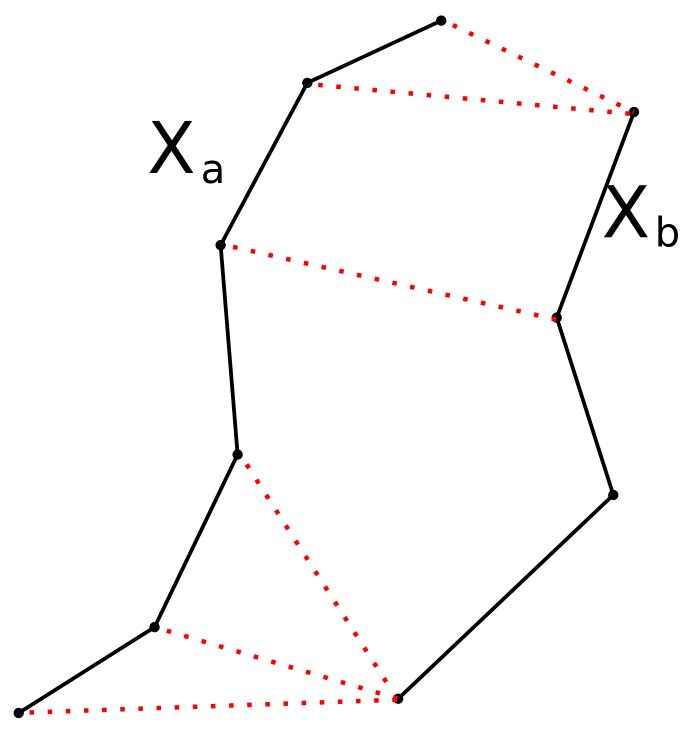
\includegraphics[width=4cm,height = 4cm]{streamline_structural_distance.pdf}
  \caption{Many distances between two streamlines, $s_A$ and $s_B$
    (solid line), that are proposed in the literature are based on the
    set of minimum distances between each point of $s_A$ to $s_B$.
    The set of minimal distances is represented here as dotted lines.}
  \label{fig:structural_distance}
\end{figure}

%\subsubsection{STAPLE sensitivity and specificity score}
%\label{subsec:experiments_quatification_staple}
%some text here

\subsubsection{Proposed method for hypotesting}
\label{subsec:experiments_quatification_proposedmethod}
From the prior knowledge of neuroscientists and doctors, there is an evidence about the reducing of the number of fibers in CST of ALS patient compared with control people. It is also the same situation with the volume of CST. Beside the number of fibers and the volume, FA and MD also play an important role for recognizing the ALS disease \cite{horsfield2002applications}. \cite{ellis1999diffusion} shows that along the corticospinal tracts, mean diffusivity was found to be significantly increased
$(p = 0.001)$ in ALS patients (limb onset: $0.771\times10^{-3} mm^2 s^{-1}$; bulbar onset: $0.778\times10^{-3} mm^2 s^{-1}$) compared with controls ($0.732\time10^{-3} mm^2 s^{-1}$). Fractional anisotropy was significantly reduced ($p = 0.007$) in bulbar onset subjects ($0.726$) compared with controls ($0.773$), but no significant difference was found between limb onset subjects ($0.761$) and controls.
Ellis et al.\cite{ellis1999diffusion} also demonstrated a positive correlation between mean diffusivity and disease duration ($r = 0.57; p = 0.009$) but no correlation with disease severity ($p > 0.29$) or upper motor neuron involvement. On the other hand, fractional anisotropy was found to correlate with measures of disease severity (assessed using the Ashworth spasticity scale and the ALS severity scale $29$).While there was no correlation between anisotropy and disease duration ($r = -0.17; p = 0.48$), significant correlations between anisotropy and the ALS severity scale ($r = -0.63; p = 0.003$) and Ashworth spasticity scale
($r = -0.56; p = 0.007$) existed.
Following are some features effectively affecting on ALS

\begin{itemize}
	\item fiber count: the number of DTI streamlines extracted for a fiber tract
	\item fiber min/max/mean length: length in $mm$ for all streamlines belonging to a fiber tract
	\item fiber volume: number of voxels occupied by all streamlines for a particular fiber tract or the geometry cylinder bounding a particular fiber tract
	\item fiber density: the ratio between fiber count and the number of voxel
	\item FA
	\item MD
	\item fragmentation: can be quantified by the ratio between the number of fibers and the volume
\end{itemize}
These features have been used as the measurement for the correctness of tractography in \cite{wang2012comprehensive}. To correct for individual differences in head size, fiber count and tract volume were normalized by intracranial volume, which was calculated from T1-weighted images using the SIENAX program in FSL \cite{smith2004techniques, smith2002accurate, smith2002automated}. 





